\documentclass[../main.tex]{subfiles}
\begin{document}

\section{Stitching}

Wie schon beschrieben überlappen die mithilfe des Laserscanner aufgenommen Daten.
Diese Überlappung kann benutzt werden, um die Bilder zu einem zusammenzufügen.
Für das Stitching von Bilddateien existieren schon mehrere Verfahren die in Bibliotheken
für viele Programmiersprachen implementiert sind. Der schon beschriebene ICP-Algorithmus
ist eines dieser Verfahren. Das Problem mit diesen Verfahren ist das sich zwei 
Datensätze angenähert werden indem auf ein Datensatz so lange eine 
Transformation und Rotation, manchmal auch eine Skalierung, angewendet wird, bis
die Distanz der Datensätze unter einen Grenzwert fällt oder nicht mehr verbessert
werden kann. Die Überlappung in den von dem Laserscanner aufgenommen Daten ist jedoch 
nur in zwei Achsen verschoben. Durch eine Rotation der Daten wird eine nicht korrekte 
Distanz berechnet.
Um die korrekte Transformation zu finden, mit der die beiden Bilder überlappen
muss nicht der komplette Bereich analysiert werden, sondern nur der überlappende Teil.
In diesem Bereich müssen Features erkannt werden. 
Nachdem in beiden Teilbildern Features erkannt wurden können diese miteinander
verglichen werden.

\subsection{Feature Erkennung}

Features in einem Bild sind große Unterschiede in benachbarten Pixeln. Die größten
Features sind die Ränder des Bauteils, kleinere Features können Oberflächenänderungen 
oder Spuren des Herstellungsprozesses sein. Diese Unterschiede können mithilfe 
der 'OpenCV' Bibliothek extrahiert werden. Diese Bibliothek gibt die erkannten 
Features als Liste von Konturen aus. Konturen selbst bestehen aus Listen von 
Punkten, die aus X und Y Koordinaten bestehen. Die Konturerkennung kann verbessert 
werden, indem das Bild entsprechend präpariert wird. In Abbildung \ref{fig:cons} und
\ref{fig:image_top} ist das Ursprungsbild und die extrahierten Konturen zu sehen.
Mittig am linken und rechten Rand sind in Abbildung \ref{fig:image_top} 
Messfehler des Laserscanners zu sehen. Diese werden auch als Features in 
Abbildung \ref{fig:cons} erkannt. Diese müssen entfernt werden damit die Bilder 
korrekt zusammengefügt werden können. Erfolgt dies nicht werden diese Fehler miteinander
verglichen was das Ergebnis verfälscht.

\begin{figure}[h]
    \centering
    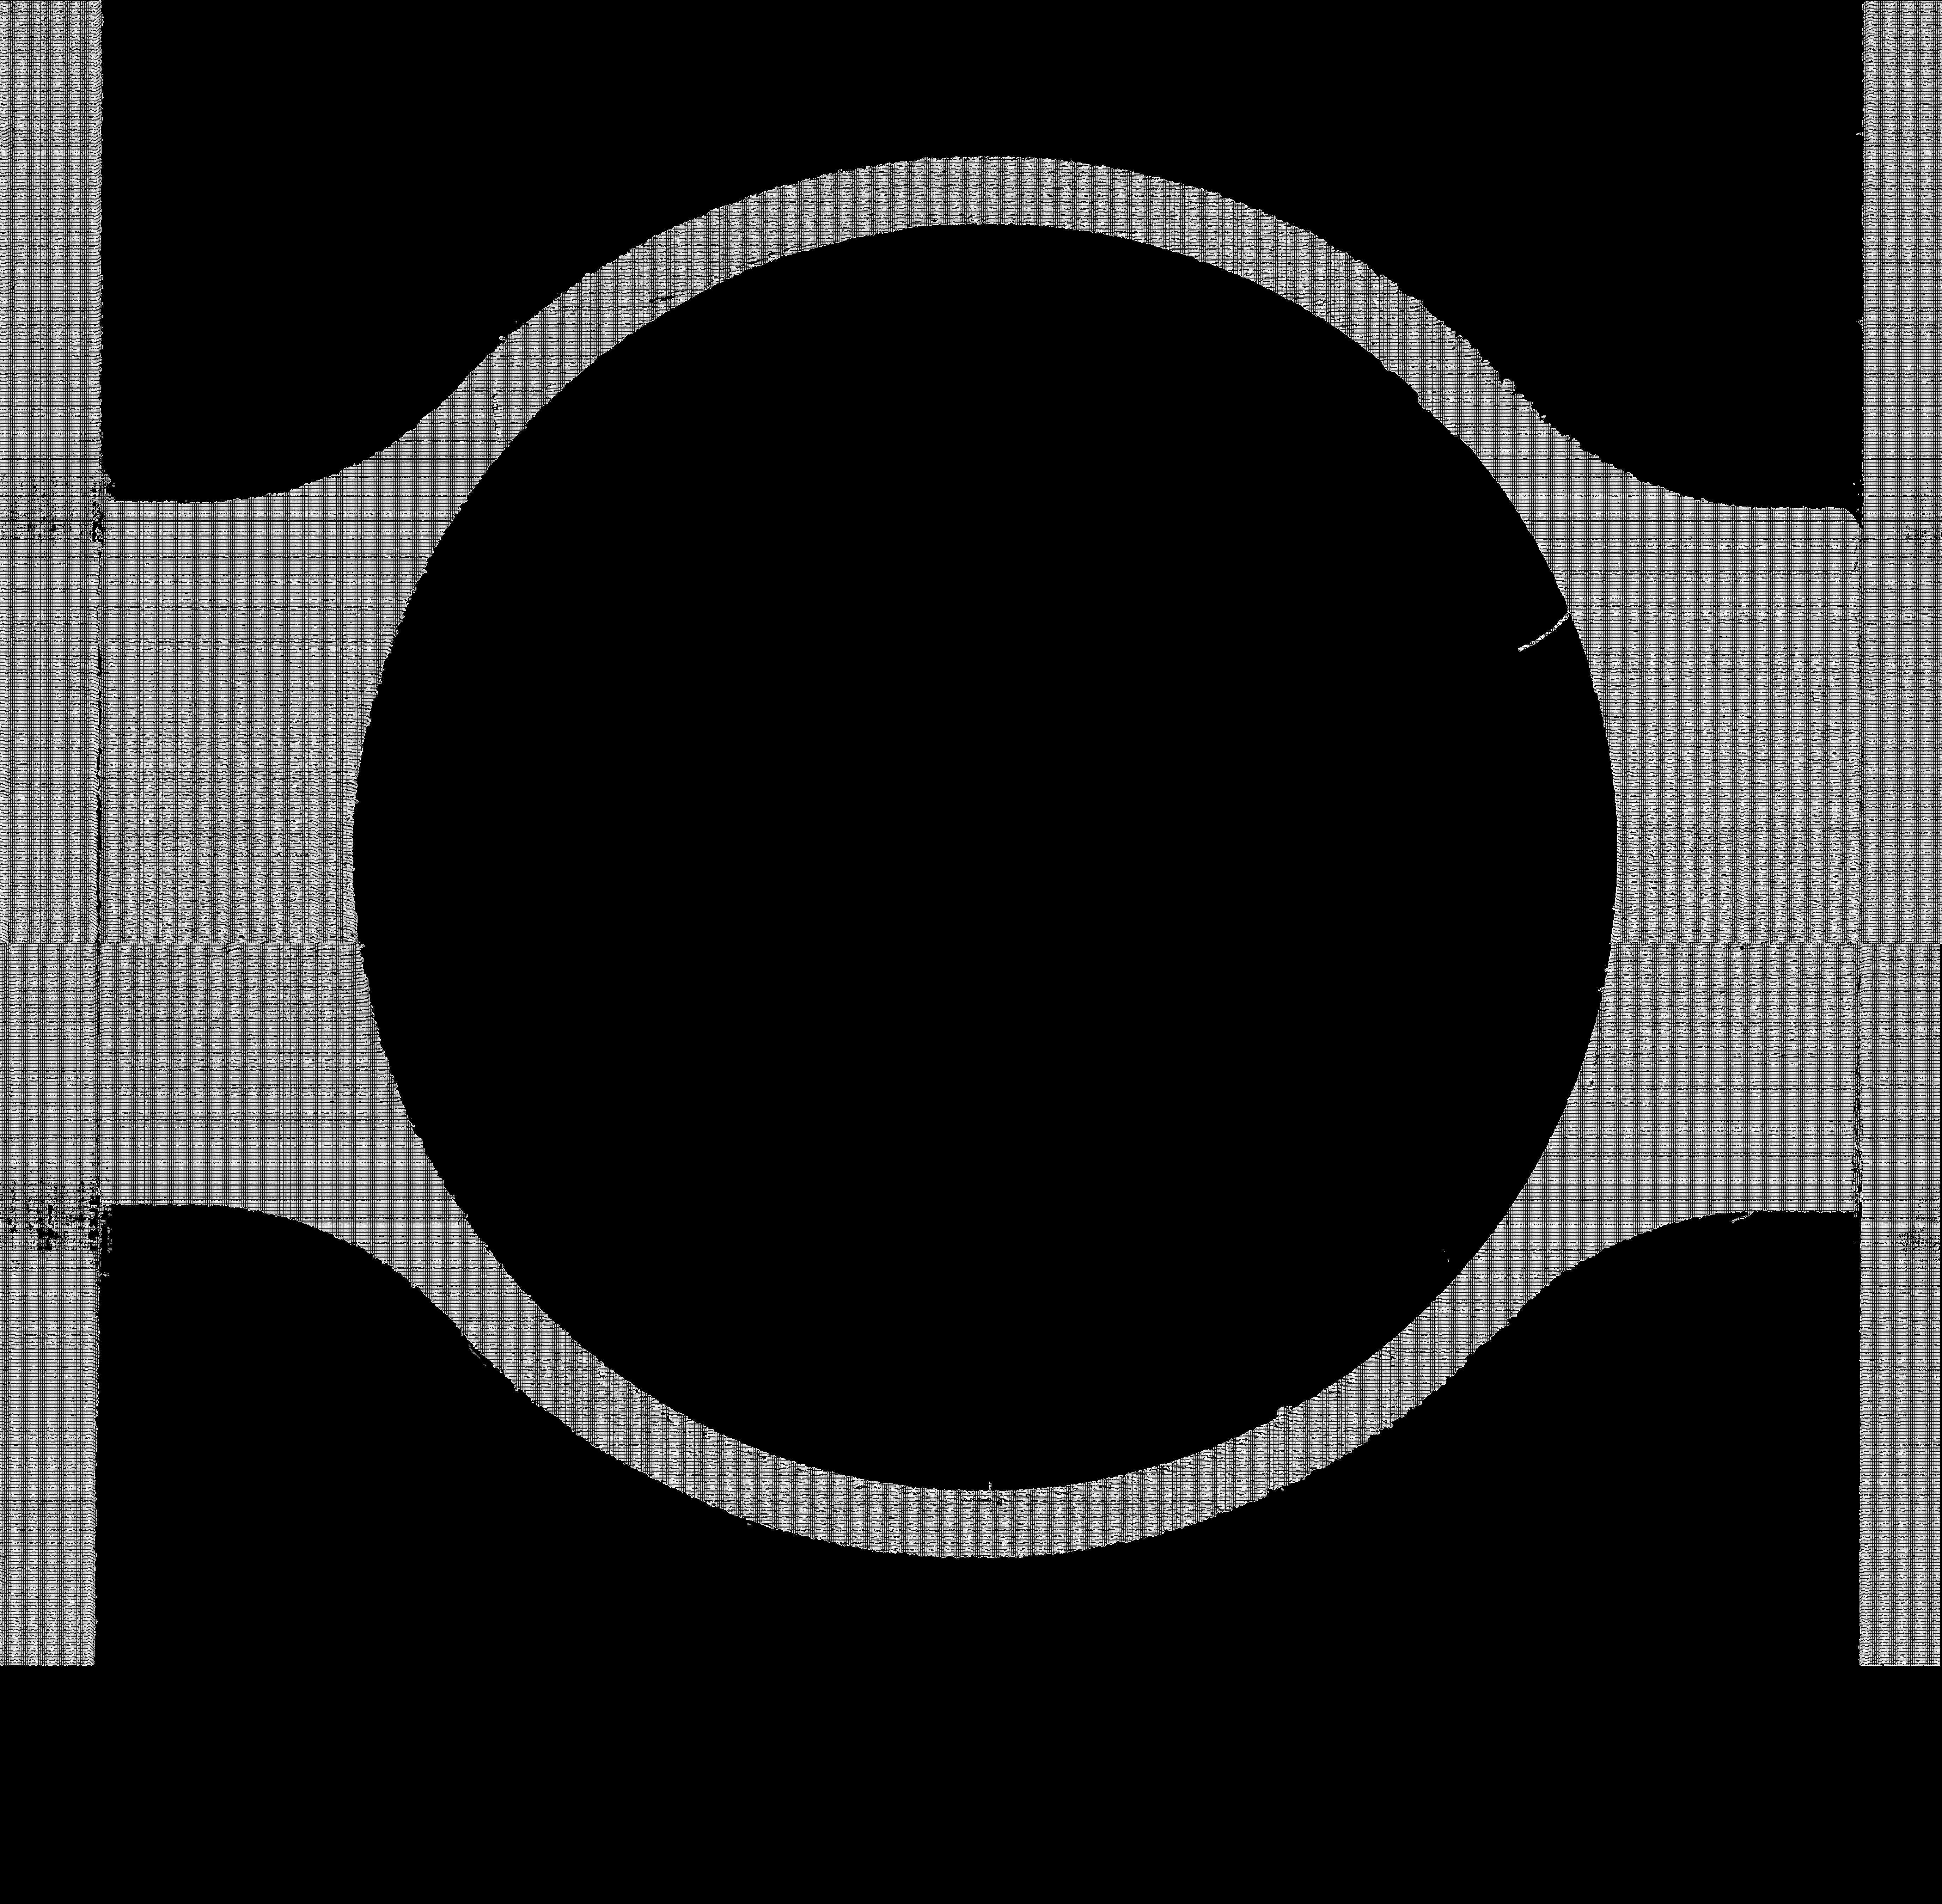
\includegraphics[width=0.8\textwidth]{images/with_con.jpg} % first figure itself
    \caption{Oberes Bild eines Scanvorgangs, FDM Bauteil}
    \label{fig:image_top}
\end{figure}

\begin{figure}[h]
    \centering
    \includegraphics[width=0.8\textwidth]{images/only_con.jpg} % second figure itself
    \caption{Extrahierte Kontouren des Bildes ohne Pre-Processing}
    \label{fig:cons}
\end{figure}

Die Überlappung kann nur im oberen oder unteren Bildbereich auftreten. Der restliche 
Teil des Bildes kann also entfernt werden. So wird außerdem Rechenzeit gespart.

\begin{figure}[h]
    \centering
    \includegraphics[width=0.8\textwidth]{images/only_con_cut.jpg} % second figure itself
    \caption{Extrahierte Kontouren des Bildes ohne Pre-Processing, zugeschnitten 
    auf den (vermutlich) überlappenden Bereich}
    \label{fig:cons_cut}
\end{figure}

Dieses Verfahren wird auf beide Bilder angewendet. Daraus resultieren dann zwei 
zugeschnittene Bilder aus denen Konturen extrahiert wurden. 
Würden diese beiden Bildteile vollständig überlappen könnte jetzt der ICP-Algorithmus
angewendet werden. Dieser würde dann die korrekte Transformation berechnen in dem er 
die Konturen aus dem oberen Bild, mit denen aus dem unteren Bild vergleicht und die 
Distanz zwischen den Punkten minimiert. 
Der Grad der Überlappung ist unbekannt und kann nicht im Vorhinein bestimmt werden.
Dadurch kann der ICP-Algorithmus nicht eingesetzt werden. 
Eine andere wichtige Annahme kann aber getroffen werden: Jeweils eine Kontur aus 
dem oberen und unteren Bild haben mindestens einen gemeinsamen Punkt.


\end{document}